\begin{figure}[H]
\centering
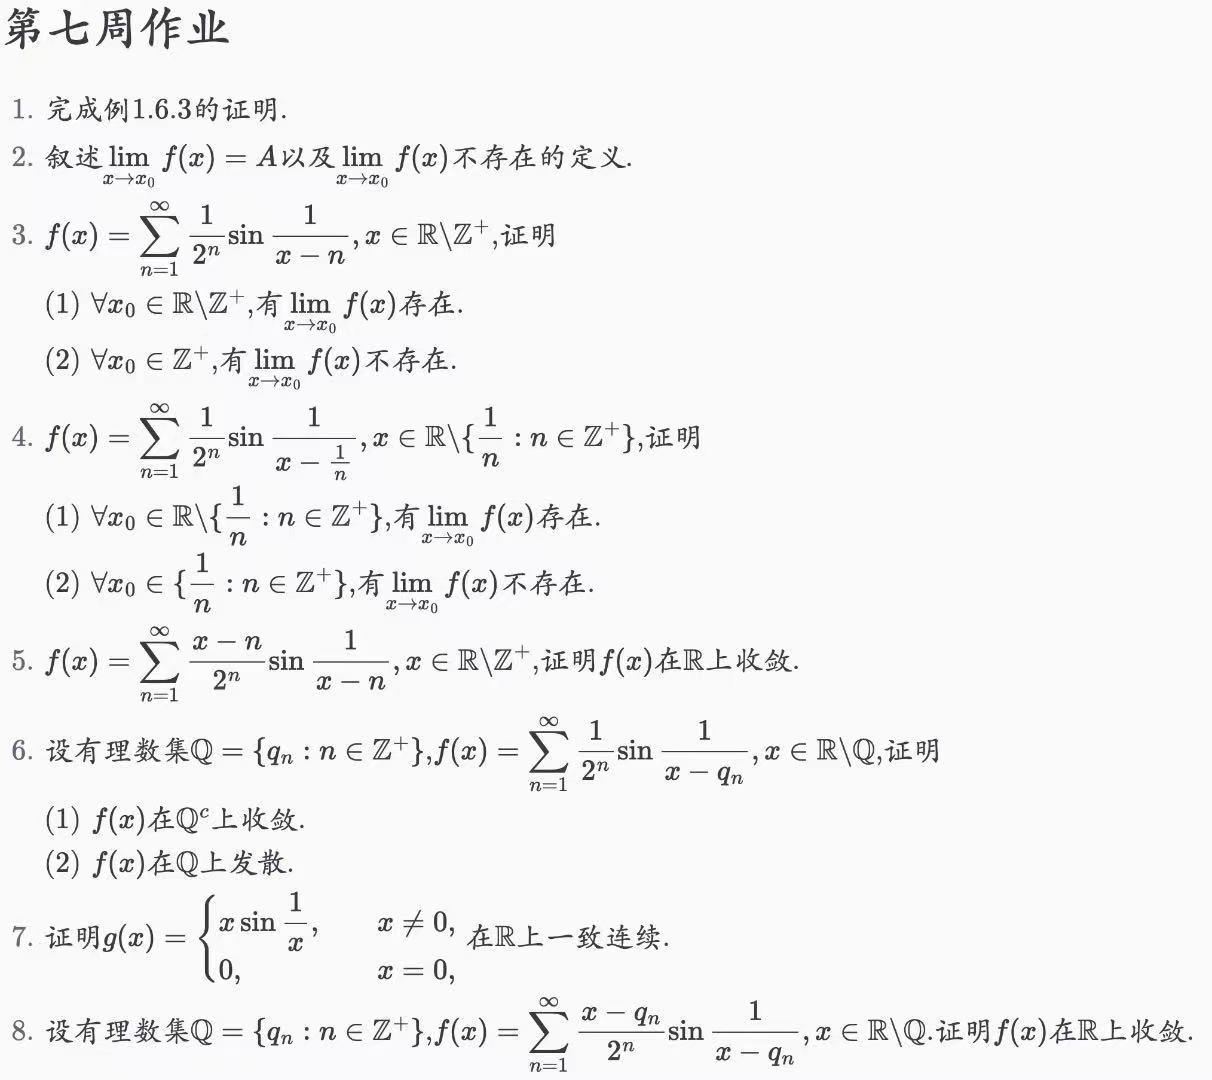
\includegraphics[width=\textwidth]{960a7c361de1ee39a977c4ad836fb639.jpg}
% \caption{}
\label{}
\end{figure}

\begin{exercise}
\begin{figure}[H]
\centering
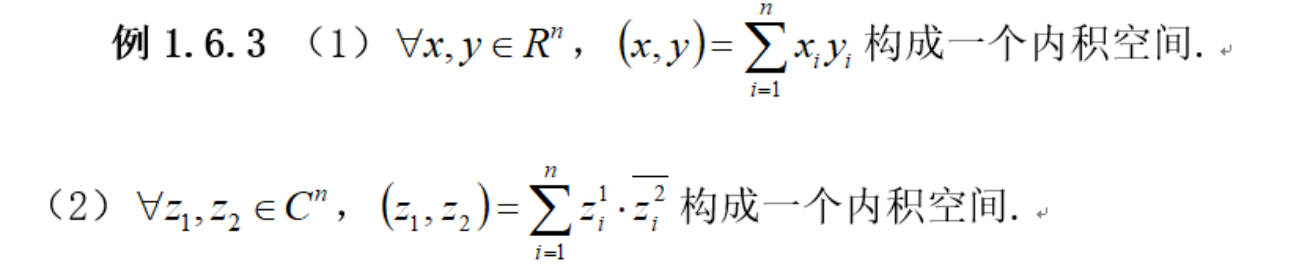
\includegraphics[width=\textwidth]{1-hw7-2025041516.png}
% \caption{}
\label{}
\end{figure}
\end{exercise}
\begin{definition}[inner product space]
\begin{figure}[H]
\centering
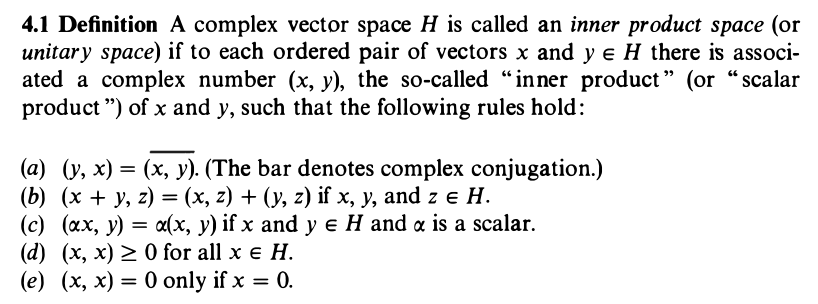
\includegraphics[width=\textwidth]{2-hw7-2025041516.png}
% \caption{}
\label{}
\end{figure}
\end{definition}
\begin{proof}
(1) Let
\[
(x,y)\coloneqq \sum_{i=1}^{n} x_iy_i \qquad \text{where }x,y\in \mathbb{R}^{n}
\]
Then for any $x, y, z\in \mathbb{R}^{n}$, $\alpha$ a scalar, we have
\[
(y,x)=\sum_{i=1}^{n} y_ix_i=\underbrace{ \sum_{i=1}^{n} x_iy_i }_{ \in \mathbb{R} }=\overline{\sum_{i=1}^{n} x_iy_i}=\overline{(x,y)}
\]
\[
(x+y,z)=\sum_{i=1}^{n} (x_i+y_i)z_i=\sum_{i=1}^{n} x_iz_i+\sum_{i=1}^{n} y_iz_i=(x,z)+(y,z)
\]
\[
(\alpha x,y)=\sum_{i=1}^{n} \alpha x_iy_i=\alpha \sum_{i=1}^{n} x_iy_i=\alpha(x,y)
\]
\[
(x,x)=\sum_{i=1}^{n} x_i^2\geq 0
\]
Let $(x,x)=0$ then
\[
\sum_{i=1}^{n} x_i^2=0\iff x_i=0,\forall i\in \{ 1,2,\dots,n \}\iff x=0
\]
(2)
Let
\[
(z_1,z_2)=\sum_{j=1}^{n} z^{1}_j\cdot  \overline{z^{2}_{j}}\qquad \text{where }z_1,z_2\in \mathbb{C}^{n}
\]
Then for any $x, y, z\in \mathbb{C}^{n}$, scalar $\alpha$, we have
\[
(y,x)=\sum_{j=1}^{n} y_j \overline{x_j}=\overline{\sum_{j=1}^{n} x_j \overline{y_j}}=\overline{(x,y)}
\]
\[
(x+y,z)=\sum_{j=1}^{n} (x_j+y_j)\overline{z_j}=\sum_{j=1}^{n} x_j \overline{z_j}+\sum_{j=1}^{n} y_j \overline{z_j}=(x,z)+(y,z)
\]
\[
(\alpha x,y)=\sum_{j=1}^{n} \alpha x_j \overline{y_j}=\alpha \sum_{j=1}^{n} x_j \overline{ y_j}=\alpha(x,y)
\]
\[
(x,x)=\sum_{j=1}^{n} x_j \overline{x_j}=\sum_{j=1}^{n} \lvert x_j \rvert ^2\geq 0
\]
\[
(x,x)=0\iff \sum_{j=1}^{n} \lvert x_j \rvert ^2=0\iff \lvert x_j \rvert ^2=0,\forall j\iff x_j=0,\forall j\iff x=0
\]
\end{proof}

\begin{exercise}
\begin{figure}[H]
\centering
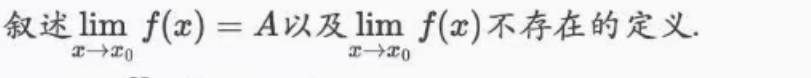
\includegraphics[width=\textwidth]{hw7-2025041517.png}
% \caption{}
\label{}
\end{figure}
\end{exercise}
\begin{figure}[H]
\centering
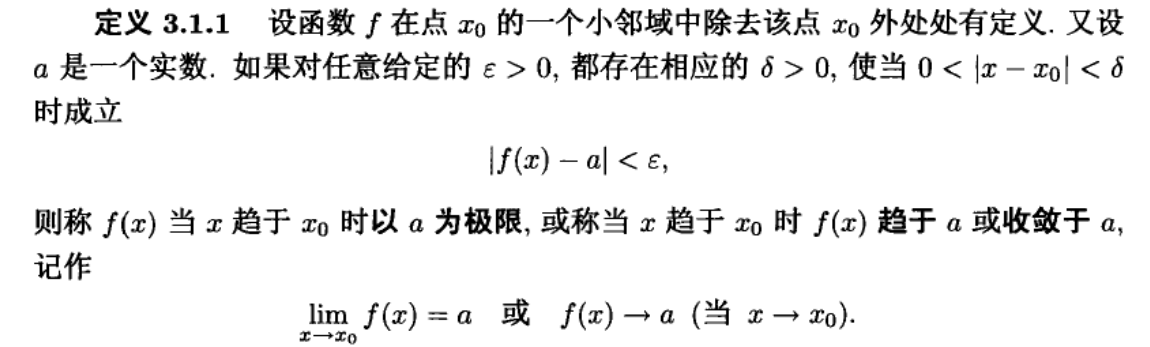
\includegraphics[width=\textwidth]{hw7-2025041616.png}
% \caption{}
\label{}
\end{figure}
$\lim_{ x \to x_0 }f(x)=A$ means for any $\epsilon>0$, there exists $\delta>0$ s.t. for any $x$ satisfying $\lvert x-x_0 \rvert<\delta$, we have
\[
\lvert f(x)-A \rvert <\epsilon
\]
$\lim_{ x \to x_0 }$ not existing means that there exists $\epsilon_0>0$, for any $\delta>0$, there exists $x_1,x_2$ satisfying $\lvert x_1-x_0 \rvert<\delta,\lvert x_2-x_0 \rvert<\delta$ and
\[
\lvert f(x_1)-f(x_2) \rvert >\epsilon_0
\]
\begin{exercise}
\begin{figure}[H]
\centering
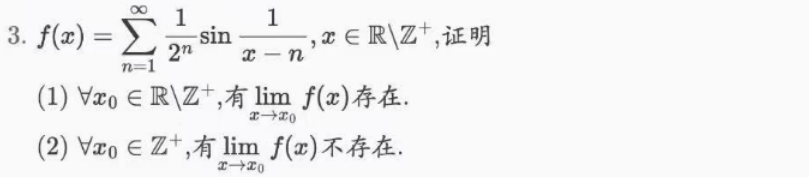
\includegraphics[width=\textwidth]{1-hw7-2025041517.png}
% \caption{}
\label{}
\end{figure}\label{f5f813}
\end{exercise}

\begin{proof}
(1) Pick any sequence $\{ x_k \}_{k=1}^{\infty}\to x_0$, $x_k\neq x_0,\forall k$. Denote $\delta=\inf_{n\in \mathbb{Z}^{+}}\lvert x_0-n \rvert$. For any $\epsilon>0$, there exists $K>0$, s.t.
\[
\lvert x_0-x_k \rvert <\min\left( \frac{\delta}{2},\frac{\epsilon\delta^{2}}{4} \right)\qquad \forall k\geq K
\]
Then
\[
\lvert x_k-n \rvert \geq \lvert x_0-n \rvert -\lvert x_0-x_k \rvert \geq \frac{\delta}{2}\qquad \forall k\geq K
\]
For any $k, k'\geq K$, we have
\[
\begin{aligned}
\lvert f(x_k)-f(x_{k'}) \rvert  & \leq \sum_{n=1}^{\infty} \frac{1}{2^{n}}\left\lvert  \sin\frac{1}{x_k-n} -\sin\frac{1}{x_{k'}-n}   \right\rvert  \\
 & \leq \sum_{n=1}^{\infty} \frac{1}{2^{n}}\left\lvert  \frac{1}{x_k-n}-\frac{1}{x_{k'}-n}  \right\rvert  \\
 & =\sum_{n=1}^{\infty} \frac{1}{2^{n}}\cdot\frac{\lvert x_k-x_{k'} \rvert }{\lvert (x_k-n)(x_{k'}-n) \rvert } \\
 & \leq \sum_{n=1}^{\infty} \frac{1}{2^{n}}\cdot  \frac{\epsilon\delta^{2}/4 }{(\delta/2)^2} \\
 & =\sum_{n=1}^{\infty} \frac{1}{2^{n}}\cdot\epsilon \\
 & =\epsilon
\end{aligned}
\]
Thus $\{ f(x_k) \}_{k=1}^{\infty}$ converges. By Heine's theorem,
\[
\lim_{ x \to x_0 } f(x)
\]
exists.

(2) When $n=x_0$, we have
\[
f(x)\underbrace{ =\sum_{n<x_0}\frac{1}{2^{n}}\sin\frac{1}{x-n} }_{ \eqqcolon A }+\underbrace{ \frac{1}{2^{x_0}}\sin\frac{1}{x-x_0} }_{ \eqqcolon B }+\underbrace{ \sum_{n>x_0}\frac{1}{2^{n}}\sin\frac{1}{x-n} }_{ \eqqcolon C }
\]
Let $x\to x_0$, we have
\[
\left\lvert  A -\sum_{n<x_0}\frac{1}{2^{n}}\sin\frac{1}{x_0-n} \right\rvert\leq \sum_{n<x_0}\frac{1}{2^{n}}\frac{\lvert x-x_0 \rvert }{\lvert (x-n)(x_0-n) \rvert }\leq \sum_{n<x_0}\frac{\lvert x-x_0 \rvert }{2^{n}}\leq  \lvert x-x_0 \rvert \to0
\]
\[
\left\lvert  C-\sum_{n>x_0}\frac{1}{2^{n}}\sin\frac{1}{x_0-n}  \right\rvert \leq  \sum_{n>x_0}\frac{1}{2^{n}}\frac{\lvert x-x_0 \rvert }{\lvert (x-n)(x_0-n) \rvert }\leq \sum_{n>x_0}\frac{\lvert x-x_0 \rvert }{2^{n}}\leq  \lvert x-x_0 \rvert \to0
\]
Let $x_m=x_0+\frac{1}{2m\pi+\frac{\pi}{2}},y_m=x_0+\frac{1}{2m\pi-\frac{\pi}{2}}$ then $x_m,y_m\to x_0$, as $m\to \infty$. But
\[
\left\lvert  \frac{1}{2^{x_0}}\sin\frac{1}{x_m-x_0}-\frac{1}{2^{x_0}}\sin\frac{1}{y_m-x_0}  \right\rvert =\left\lvert  \frac{1}{2^{x_0}}+\frac{1}{2^{x_0}}  \right\rvert =\frac{1}{2^{x_0-1}}\centernot{\to}0\qquad \text{as }m\to \infty
\]
Thus $\lim_{ x \to x_0 }B$ does not exists, while $\lim_{ x \to x_0 }A$ exists, $\lim_{ x \to x_0 }C$ exists. Hence
\[
\lim_{ x \to x_0 } f(x)
\]
does not exists.
\end{proof}

\begin{exercise}
\begin{figure}[H]
\centering
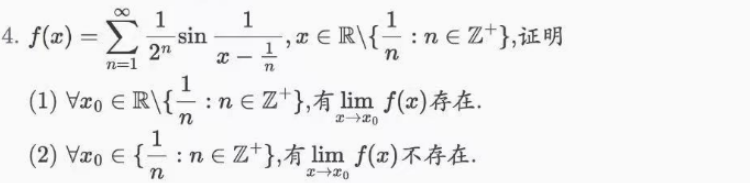
\includegraphics[width=\textwidth]{3-hw7-2025041517.png}
% \caption{}
\label{}
\end{figure}
\end{exercise}
\begin{figure}[H]
\centering
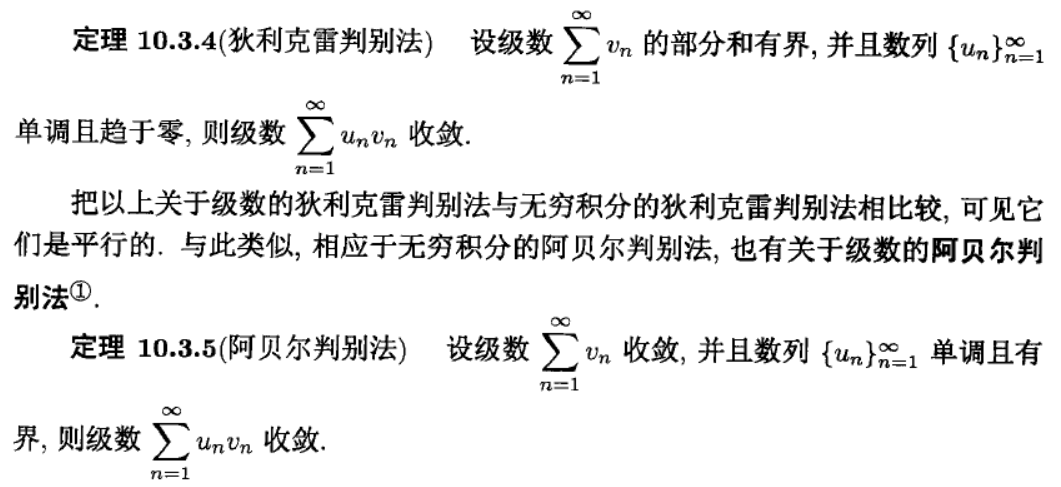
\includegraphics[width=\textwidth]{1-hw7-2025041616.png}
% \caption{}
\label{}
\end{figure}

\begin{proof}
(1) for any $x_0\in \mathbb{R}\setminus \left\{  \frac{1}{n}:n\in \mathbb{Z}^{+}  \right\}$, check that
\[
\lim_{ x \to x_0 } f(x)=\sum_{n=1}^{\infty} \frac{1}{2^{n}}\sin\frac{1}{x_0-\frac{1}{n}}
\]
因为 $\sin\frac{1}{x_0-\frac{1}{n}}$ 关于充分大的 $n$ 单调有界趋于 $\sin\frac{1}{x_0}$,且级数 $\sum_{n=1}^{\infty}\frac{1}{2^{n}}=1$ 收敛. 由 Abel test,级数 $\sum_{n=1}^{\infty}\frac{1}{2^{n}}\sin\frac{1}{x_0-\frac{1}{n}}$ 收敛.

(2) 任意给定 $x_0\in \left\{  \frac{1}{n}:n\in \mathbb{Z}^{+}  \right\}$,则
\[
f(x)=\sum_{n<x_0 ^{-1}}\frac{1}{2^{n}}\sin\frac{1}{x-\frac{1}{n}}+\frac{1}{2^{x_0^{-1}}}\sin\frac{1}{x-x_0}+\sum_{n>x_0 ^{-1}}\frac{1}{2^{n}}\sin\frac{1}{x-\frac{1}{n}}
\]
令 $x\to x_0$,那么下面两个级数收敛
\[
\sum_{n<x_0 ^{-1}}\frac{1}{2^{n}}\sin\frac{1}{x-\frac{1}{n}}\to \sum_{n<x_0 ^{-1}}\frac{1}{2^{n}}\sin\frac{1}{x_0-\frac{1}{n}}
\]
\[
\sum_{n>x_0 ^{-1}}\frac{1}{2^{n}}\sin\frac{1}{x-\frac{1}{n}}\to \sum_{n>x_0 ^{-1}}\frac{1}{2^{n}}\sin\frac{1}{x_0-\frac{1}{n}}
\]
考虑数列 $\left\{  x_k=x_0+\frac{1}{2k\pi+\frac{\pi}{2}}  \right\}_{k=1}^{\infty},\left\{  y_k=x_0+\frac{1}{2k\pi-\frac{\pi}{2}}  \right\}_{k=1}^{\infty}$,于是
\[
\left\lvert  \frac{1}{2^{x_0 ^{-1}}}\sin\frac{1}{x_k-x_0}-\frac{1}{2^{x_0 ^{-1}}}\sin\frac{1}{y_k-x_0}  \right\rvert =\left\lvert  -\frac{1}{2^{x_0 ^{-1}}}-\frac{1}{2^{x_0 ^{-1}}}  \right\rvert =2^{1-x_0 ^{-1}}\centernot{\to}0
\]
故 $\lim_{ x \to x_0 }f(x)$ 不存在.

\end{proof}

\begin{exercise}
\begin{figure}[H]
\centering
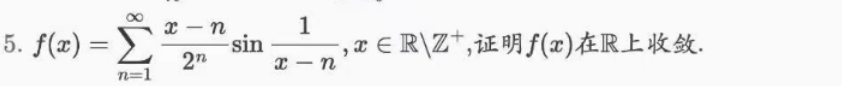
\includegraphics[width=\textwidth]{4-hw7-2025041517.png}
% \caption{}
\label{}
\end{figure}
\end{exercise}
\begin{figure}[H]
\centering
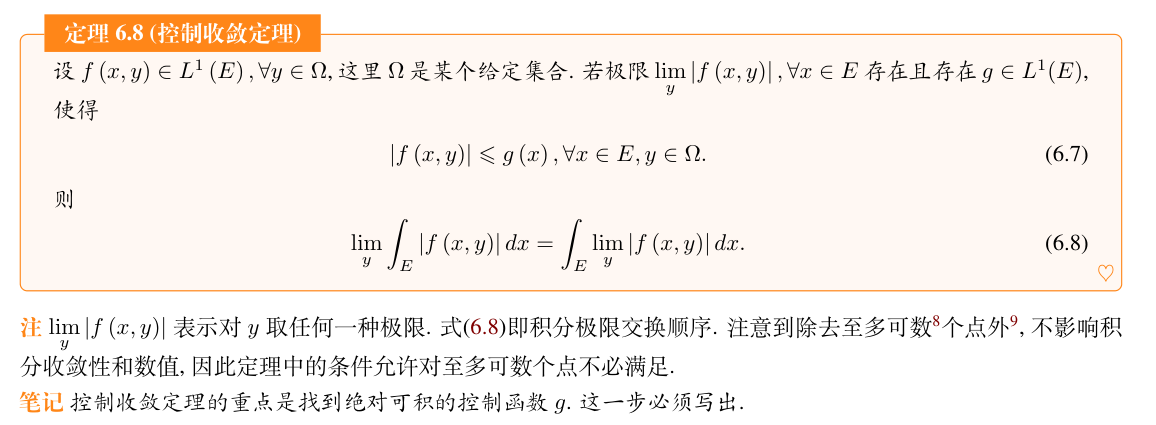
\includegraphics[width=\textwidth]{3-hw7-2025041616.png}
% \caption{}
\label{}
\end{figure}

\begin{proof}
For any given $x_0\in \mathbb{R}$, $n\in \mathbb{Z}^{+}$, the limit
\[
\lim_{ x \to x_0 }\frac{x-n}{2^{n}}\sin\frac{1}{x-n}=\begin{cases}
\frac{x_0-n}{2^{n}}\sin\frac{1}{x_0-n} & x_0\neq n \\
\frac{1}{2^{n}} & x_0=n
\end{cases}
\]
exists. And
\[
\left\lvert  \frac{x-n}{2^{n}}\sin\frac{1}{x-n}  \right\rvert \leq \frac{1}{2^{n}}\qquad \forall n\in \mathbb{N},x\in \mathbb{R}\setminus \mathbb{Z}^{+}
\]
Then
\[
\begin{aligned}
\lim_{ x \to x_0 } \sum_{n=1}^{\infty} \frac{x-n}{2^{n}}\sin\frac{1}{x-n} & =\sum_{n=1}^{\infty} \lim_{ x \to x_0 } \frac{x-n}{2^{n}}\sin\frac{1}{x-n} \\
 & =\begin{cases}
\sum_{n=1}^{\infty} \frac{1}{2^{n}}=1 & x_0\in \mathbb{Z}^{+} \\
\sum_{n=1}^{\infty} \frac{x_0-n}{2^{n}}\sin\frac{1}{x_0-n} & x_0\in \mathbb{R}\setminus \mathbb{Z}^{+}
\end{cases}
\end{aligned}
\]
i.e. the limit $\lim_{ x \to x_0 }f(x)$ exists, i.e. $f$ converges on $\mathbb{R}$ .

\end{proof}

\begin{exercise}
\begin{figure}[H]
\centering

\includegraphics[width=\textwidth]{5-hw7-2025041517.png}
% \caption{}
\label{}
\end{figure}
\end{exercise}
\begin{proof}
(1)
For any $x_0\in \mathbb{Q}^{c}$, for given $n\in \mathbb{Z}^{+}$, $\lim_{ x \to x_0 }\frac{1}{2^{n}}\sin\frac{1}{x-q_n}=\frac{1}{2^{n}}\sin\frac{1}{x_0-q_n}$ exists. And
\[
\left\lvert  \frac{1}{2^{n}}\sin\frac{1}{x-q_n}  \right\rvert \leq \frac{1}{2^{n}}
\]
By dominate convergence theorem, $f(x)$ converge on $\mathbb{Q}^{c}$.

(2)
Let $x\to x_0\in \mathbb{Q}$, then
\[
f(x)=\underbrace{ \sum_{q_n<x_0}\frac{1}{2^{n}}\sin\frac{1}{x-q_n} }_{ \text{converges} }+\underbrace{ \sum_{q_n=x_0}\frac{1}{2^{n}}\sin\frac{1}{x-q_n} }_{ \text{diverges} }+\underbrace{ \sum_{q_n>x_0}\frac{1}{2^{n}}\sin\frac{1}{x-q_n} }_{ \text{converges} }
\]
Thus $f(x)$ diverges on $\mathbb{Q}$.

\end{proof}

\begin{exercise}
\begin{figure}[H]
\centering
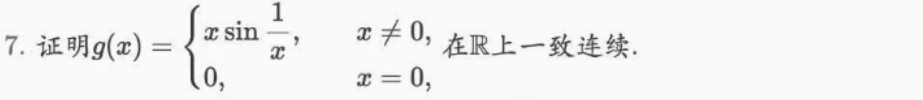
\includegraphics[width=\textwidth]{hw7-2025041518.png}
% \caption{}
\label{}
\end{figure}
\end{exercise}
\begin{proof}
Pick any $\delta>0$ then for any $x,y>\delta$, we have
\[
\begin{aligned}
\left\lvert  x\sin\frac{1}{x}-y\sin\frac{1}{y}  \right\rvert  & \leq \lvert x-y \rvert \left\lvert  \sin\frac{1}{x}  \right\rvert +\lvert y \rvert \left\lvert  \sin\frac{1}{x}-\sin\frac{1}{y}  \right\rvert  \\
 & \leq \lvert x-y \rvert +\lvert y \rvert \cdot\frac{\lvert x-y \rvert }{\lvert xy \rvert } \\
 & \leq \lvert x-y \rvert \cdot (1+1/\delta) \to0\qquad \text{as }\lvert x-y \rvert \to0
\end{aligned}
\]
Similar for $x,y<-\delta$, then $g$ is uniformly continuous on $(-\infty,-\delta)\cup(\delta,+\infty)$.

For any $\epsilon>0$, pick $\delta=\frac{\epsilon}{4}$ then for any $\lvert x \rvert,\lvert y \rvert\leq2\delta$, we have
\[
\left\lvert  x\sin\frac{1}{x}-y\sin\frac{1}{y}  \right\rvert \leq \lvert x \rvert +\lvert y \rvert \leq \epsilon
\]
Thus $g$ is uniformly continuous on $[-2\delta,2\delta]$. Hence $g$ is uniformly continuous on $\mathbb{R}$.
\end{proof}

\begin{exercise}
\begin{figure}[H]
\centering

\includegraphics[width=\textwidth]{1-hw7-2025041518.png}
% \caption{}
\label{}
\end{figure}
\end{exercise}
\begin{proof}
For any $x_0\in \mathbb{R}$, for any given $n\in \mathbb{Z}^{+}$ we have
\[
\lim_{ x \to x_0 } \frac{x-q_n}{2^{n}}\sin\frac{1}{x-q_n}=\begin{cases}
\frac{1}{2^{n}}(x_0-q_n)\sin\frac{1}{x_0-q_n} & x_0\neq q_n \\
\frac{1}{2^{n}} & x_0=q_n
\end{cases}
\]
exists.
\[
\left\lvert  \frac{x-q_n}{2^{n}}\sin\frac{1}{x-q_n}  \right\rvert \leq \frac{1}{2^{n}}
\]
By dominate convergence theorem, $f(x)$ converge on $\mathbb{R}$.
\end{proof}
